\documentclass[a4paper,14pt]{extarticle} % тип документа
\usepackage{extsizes}
\usepackage[left=3cm,right=1.5cm,top=2cm,bottom=2cm,bindingoffset=0cm,nohead]{geometry}
\usepackage{indentfirst}
\usepackage{cmap}
\usepackage[T2A]{fontenc}			% кодировка
\usepackage[utf8]{inputenc}			% кодировка исходного текста
\usepackage[english,russian]{babel}	% локализация и переносы
\usepackage{amsmath,amsfonts,amssymb,amsthm,mathtools,array} 
\usepackage{wasysym}
\usepackage[labelsep=endash]{caption}
\usepackage{graphicx}
\usepackage{pgfplots}
\usepackage{makeidx}
\usepackage{tikz}
\usepackage{pgfplots}
\pgfplotsset{compat=1.18}
\usepackage{pdfpages}
\usepackage[nottoc]{tocbibind}
\usepackage{setspace}
\linespread{1.3}
\usepackage{nomencl}
\makenomenclature
\usepackage{totcount}
\usepackage{subcaption}
\usepackage{listings}
\usepackage{diagbox}
\usepackage{placeins}
\usepackage{url}
\usepackage[colorlinks=false]{hyperref}
\usepackage{enumitem}
\usepackage{float}
\usepackage{afterpage}
% \usepackage{subfigure}
\newcommand\blankpage{%
    \null
    \thispagestyle{empty}%
    %\addtocounter{page}{-1}%
    \newpage}
% \renewcommand{\baselinestretch}{1.5} 
\regtotcounter{figure}
\regtotcounter{page}
\renewcommand{\nomname}{Сокращения и обозначения}
\newtotcounter{citnum}
\def\oldbibitem{} \let\oldbibitem=\bibitem
\def\bibitem{\stepcounter{citnum}\oldbibitem}
\newtotcounter{citesnum}
\def\oldcite{} \let\oldcite=\cite
\def\cite{\stepcounter{citesnum}\oldcite}
\makeatletter
\def\@biblabel#1{#1 }
\makeatother
\usepackage{chngcntr}
\counterwithin{figure}{section} % рисунки
\counterwithin{table}{section} % таблицы


% \newcounter{mycitecount}                                %% Счётчик библиографии
% \AtEveryBibitem{\stepcounter{mycitecount}}              %% Работает для biblatex

% \usepackage[chaptercount,%
%             figure,      %
%             table,       %
%             apxcount,    %
%             basepage,    %
%             mycitecount, xspace ]{totalcount}           %% Подсчёт общего количества объектов в документе

\author{Кузнецов Игорь}
\title{}
\date{\today}

\renewcommand{\bottomfraction}{1.0} % часть страницы, которую может занимать графика снизу страницы

\newcolumntype{L}{>{$}l<{$}} % math-mode version of "l" column type
\newcommand{\ZE}{\bar{E}}
\newcommand{\BE}{\partial E}
\newcommand{\CE}{\complement E}
\newcommand{\IE}{\stackrel{\circ}{E}}
\newcommand{\Def}{\textbf{Определение }}
\newcommand{\Ter}{\textbf{Теорема }}
\newcommand{\Utv}{\textbf{Утверждение }}
\newcommand{\Prd}{\textbf{Предложение }}
\newcommand{\Dvo}{\textbf{Доказательство }}
\newcommand{\Imp}{\textbf{(!) }}
\newcommand{\Sld}{\textbf{Следствия: }}
\newcommand{\Svv}[1]{\textbf{Свойства #1:} }
% \newcommand{\eqref}[1]{(\ref{#1})}
\DeclareMathOperator{\Ree}{Re}
\DeclareMathOperator{\Imm}{Im}
\DeclareMathOperator{\res}{res}
\DeclareMathOperator{\cov}{cov\,}
\DeclareMathOperator{\kH}{\text{кН}}
\DeclareMathOperator{\m}{\text{м}}
\DeclareMathOperator{\kHm}{\kH\cdot\m}

\begin{document}
\def\figurename{Рисунок}
% \maketitle
\newcommand{\brv}[1]{{\left| #1 \right|}}
\newcommand{\brr}[1]{{\left( #1 \right)}}
\newcommand{\brs}[1]{{\left[ #1 \right]}}
\newcommand{\brc}[1]{{\left\{ #1 \right\}}}
\newcommand{\brn}[1]{{\left\lVert #1 \right\rVert}}
\newcommand{\bra}[1]{{\left\langle #1 \right\rangle}}
\newcommand{\brrl}[1]{{\left( #1 \right]}}
\newcommand{\brrr}[1]{{\left[ #1 \right)}}
\newcommand{\under}[2]{{\underset{#2}{\underbrace{#1}}}}
\newcommand{\strm}[1]{\underset{#1}{\rightarrow}}
% 
\includepdf{Отчет по практике (2).pdf}

% 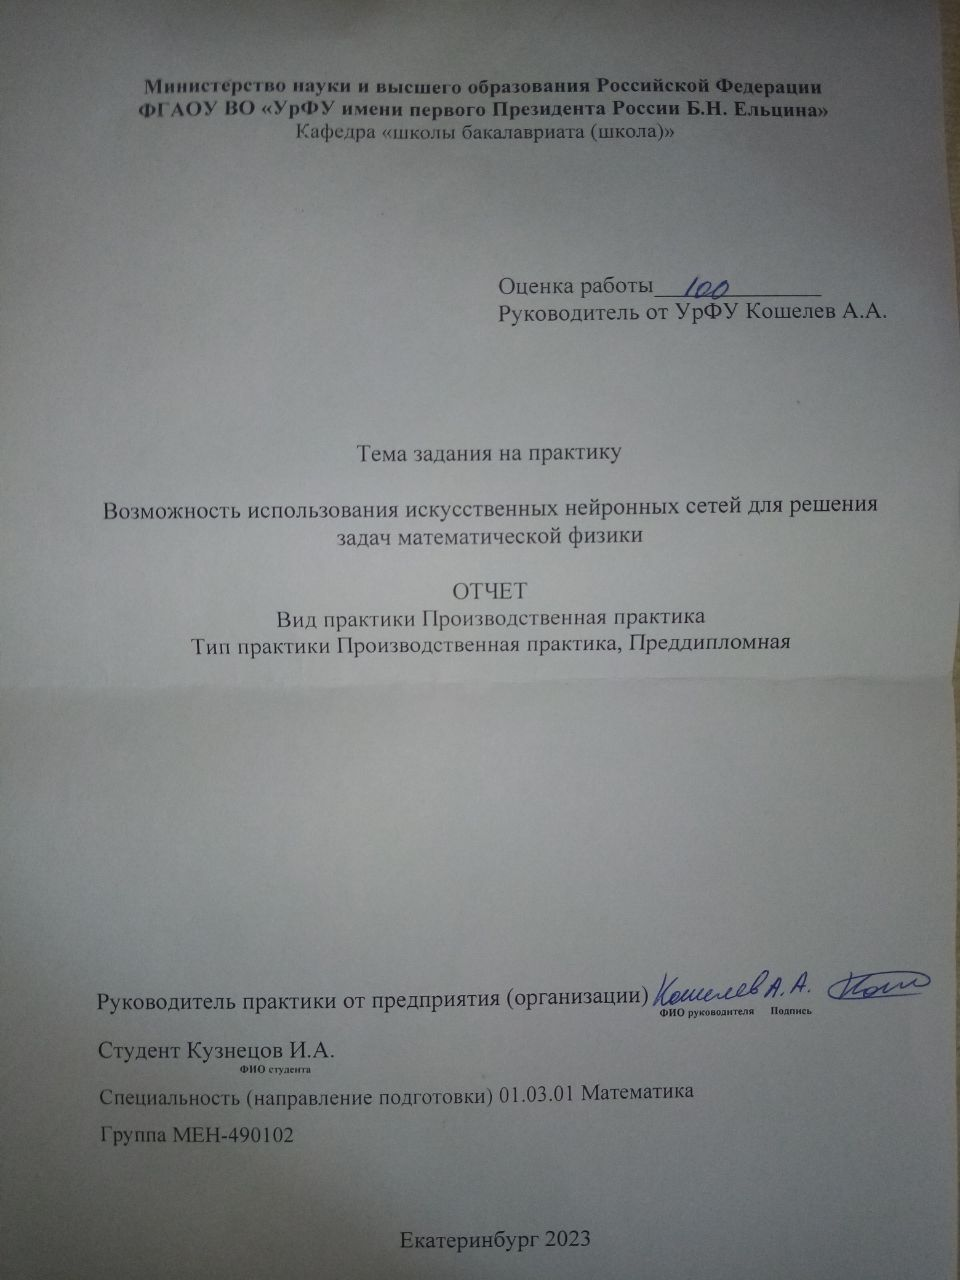
\includegraphics[width=\textwidth]{титульник.jpg}
% \afterpage{\blankpage}
% \afterpage{\null\newpage}
% \thispagestyle{empty}

\addtocounter{page}{1}%

\newpage
\begin{center}
    \section*{РЕФЕРАТ}
    \addcontentsline{toc}{section}{РЕФЕРАТ}
\end{center}

Кузнецов Игорь александрович <<Возможность использования искусственных нейронных сетей для решения задач математической физики>>:  работа содержит: страниц \total{page}, иллюстраций \total{figure}, таблиц 2, использованных источников \total{citnum}

\noindent Ключевые слова: PINN, дифференциальные уравнения, нейронные сети, Python %, численные методы

% Целью работы является исследование возможности применения PINN (Physics-Informed Neural Networks) в решении задач 
PINN (Physics-Informed Neural Networks) - это метод, который сочетает в себе преимущества нейронных сетей и физических моделей для решения задач научного моделирования. В данном дипломном проекте исследуется применение метода PINN для решения задачи установившегося распределения тепла в кольце и задачу электрокинетики. В работе проводится анализ эффективности точности и скорости метода PINN. Также исследуется влияние различных параметров на точность рения задачи и высказаны идеи по улучшению полученных результатов. Результаты исследования показывают, что метод PINN может решить простую задачу с кольцом, однако боле сложная задача электрокинетики, решается плохо. % , особенно в случаях, когда классические методы неэффективны или недостаточно точны.
Для решения задачи были использованы следующие технологии:
\begin{enumerate}[label={\arabic*)}]
    \item язык программирования Python
    \item библиотека для работы с глубокими нейронными сетями Tensorflow
\end{enumerate}

\newpage
\tableofcontents

% \section*{Обозначения и сокращения}

В настоящей работе применяют следующие обозначения и сокращения

\begin{description}
    \item[PINN] -- Physics-Informed neural network, физически информированная нейронная сеть
    \item[$c$] -- Концентрация ионных частиц
    \item[$j$] -- Поток плотности
    \item[$\vec{v}$] -- Адвективная скорость жидкости
    \item[$e$] -- Заряд электрона
    \item[$z$] -- Валентность частиц
    \item[$\Phi$] -- Электростатический потенциал
    \item[$\xi$] -- Подвижность частиц
    \item[$D$] -- Коэффициент диффузии частиц
    \item[$l_B$] -- Длина Бьеррума, $l_B = \frac{e^2}{4\pi\varepsilon k_B T}$
    \item[$k_B$] -- Постоянная Больцмана
    \item[$T$] -- Температура
    \item[$\rho$] -- Плотность жидкости
    \item[$p_H$] -- Гидродинамическое давление
\end{description}

% \noindent\begin{tabular}{llm{15cm}}
%     PINN & -- & Physics-Informed neural network, физически информированная нейронная сеть
% \end{tabular}

\newpage

% \\nomenclature \{(\$[a-z\\\{\}_]*\$)\}\{(.*)\}
% \\item[$1] -- $2
% \nomenclature {$c$}{Концентрация ионных частиц}
% \nomenclature {$j$}{Поток плотности}
% \nomenclature {$\vec{v}$}{Адвективная скорость жидкости}
% \nomenclature {$e$}{Заряд электрона}
% \nomenclature {$z$}{Валентность частиц}
% \nomenclature {$\Phi$}{Электростатический потенциал}
% \nomenclature {$\xi$}{Подвижность частиц}
% \nomenclature {$D$}{Коэффициент диффузии частиц}
% \nomenclature {$l_B$}{Длина Бьеррума, $l_B = \frac{e^2}{4\pi\varepsilon k_B T}$}
% \nomenclature {$k_B$}{Постоянная Больцмана}
% \nomenclature {$T$}{Температура}
% \nomenclature {$\rho$}{Плотность жидкости}
% \nomenclature {$p_H$}{Гидродинамическое давление}

% \printnomenclature


\newpage
\begin{center}
    \section*{ВВЕДЕНИЕ}
    \addcontentsline{toc}{section}{ВВЕДЕНИЕ}
\end{center}

В последние годы нейронные сети получили широкое распространение, они используются для анализа и генерации изображений и видео, обработки естественных языков (перевод, чат-боты), медицинской диагностике, финансовых прогнозах и так далее.

Одним из перспективных направлений в этой области являются так называемые PINN -- Physics-Informed Neural Networks, физически-инфор\-мированные нейронные сети. Классические нейронные сети используют большую выборку реальных данных, однако в естественно-научных областях, таких как физика, химия, биология и т.д. зачастую может просто не хватать нужного объёма данных для обучения. PINN способны обойти это ограничения, используя в обучении знания законов физики, описываемые дифференциальными уравнениями в частных производных. Это позволяет использовать неполные и зашумленные данные, что делает их полезными в реальных научных задачах. Однако, вычислительная сложность PINN выше, чем у классических нейронных сетей, что требует большого количества вычислительных мощностей.

\newpage
\begin{center}
    \section*{ОСНОВНАЯ ЧАСТЬ}
    \addcontentsline{toc}{section}{ОСНОВНАЯ ЧАСТЬ}
\end{center}

\section{Постановка задачи}

\subsection{Цель работы}

% Рассмотреть уже решённую физическую задачу, решить её с помощью PINN и сравнить полученные данные с изначальным решением, оценить целесообразность применения PINN к задаче.

Рассмотреть задачу распределения тепла в диске и задачу электрокинетики, решить их с помощью PINN и сравнить полученные данные с решениями, полученными другими способами, оценить целесообразность применения PINN к задаче.

\subsection{Описание задачи}

Создать нейросеть, которой на вход подаются пространственные координаты. На выходе хотим значение физической величины в данной точке. Обучить данную нейросеть используя методику PINN. Провести оценку результатов обучения: скорость, точность ответа.

\section{Обзор литературы}

% Впервые терми PINN был введён в статье \cite{bib:pinn:first}. В ней автор дал формальное определение PINN'ам и рассмотрел решение нескольких задач: уравнение Шрёдингера, Навье-Стокса, Ален-Чана.

Одна из первых работ, посвященных PINNs, была опубликована в 2019 году Мазьяром Райсси и его коллегами \cite{bib:pinn:first}. В этой работе авторы представили метод, который позволяет использовать уравнения в частных производных в качестве ограничений для обучения нейронной сети. Они показали, что этот метод может быть использован для решения широкого спектра задач, включая уравнения Навье-Стокса, уравнения Максвелла и тому подобное.

В настоящее время PINN широко применяются моделировании, анализе широкого спектра физических явлений:

В статье \cite{bib:voltogr:1} рассматривается задача симуляции циклической вольтаметрии, исследователями было рассмотрено несколько случая: одномерная вольтаметрия на дисковом электроде с полубесконечными или тонкослойными граничными условиями, двумерная вольтаметрия на микрополосковом электроде и наконец вольтаметрия на края квадратного электрода, количественно определяя неравномерное распределение тока вблизи угла электрода. Для моделирования был использован перцептрон использующий от трёх до шести скрытых слоёв, и гиперболический тангенс в качестве функции активации. Полученные исследователями данные хорошо согласуются с решениями этих же задач, полученными другими способами.

Так же PINN применяются для: анализа литий-ионных батарей\cite{bib:lbat:1,bib:lbat:2}, для моделирование теплопереноса в системах со сложной геометрией \cite{bib:heat:1,bib:heat:2}, решения уравнения Навье-Стокса для моделирования турбулентности \cite{bib:navstock:1}, химической кинематике \cite{bib:chemkin:1,bib:chemkin:2}, для решения задач оптимизации с ограничениями, таких как задачи оптимизации формы \cite{bib:grazzi2020iteration}. Для изучения биологических процессов существует разновидность PINN -- BINN (Biologically-informed neural network) \cite{bib:BINN:1}

\section{Способы и методы решения задачи}
\subsection{Нейронные сети}\label{sect:nn}

Задачу решения системы дифференциальных уравнений можно рассматривать как задачу регрессии, то есть задачу нахождения непрерывного соотношения между зависимой переменной $u$ и одной или несколькими независимыми переменными  $z = (z^1, z^2, ... z^n)^T$ по обучающей выборке $T = \brc{z_i, u_i}_{i=1}^{N_f}$ (в нашем случае начальным и граничным условиям). Следовательно нашей задачей является поиск функции $\bar{u} = \bar{u}(z, \theta)$, аппроксимирующей истинную функцию $u(z)$ для любых значений $z$. В качестве $\bar{u}$ обычно выступает нелинейная функция, определяемая соответствующим методом регрессии и зависящая от своего набора параметров $\theta=(\theta_1, \theta_2, ..., \theta_k)^T$. Набор параметров $\theta$ подбирается таким образом, что бы
\begin{equation}\label{eq:gen_loss}
    \theta=\min_\theta\brn{\bar{u}(z_i,\theta)}, i=\overline{1, N_f}.
\end{equation}

Процесс подбора этих параметров называется обучением модели.

\textbf{Определение 1.} Определим функцию регрессии $f$ следующим образом:
\begin{equation}
    f(z, \theta) = h\brr{\sum_{j=1}^p w_j z^j + b} = h(wz+b),
\end{equation}
где $h$ -- функция активации (обычно берётся сигмоида, $\tanh$ или ReLu), $w = (w_1, w_2, ... w_p)$ -- веса, $b$ -- смещение, $w$ и $b$ вместе являются параметрами $\theta$ функции $\bar{u}$, $\theta = (w_1, w_2, ..., w_p, b)^T$. % Данный вид функции регрессии называется обобщённой линейной регрессией.

\textbf{Определение 2.} Искусственной нейронной сетью называют последовательность нескольких функций из определения 1. Сеть с $L$ скрытыми слоями и $N$ нейронами на слой может быть записана следующим образом:

\begin{equation}
    \begin{aligned}
        q^{(l, n)} & = h\brr{\sum_{i=1}^N w_i^{(l,n)}q^{(l-1,i)}+b^{(l,n)}}, n=1,...,N,\; l=1,...,L-1 \\
        q^{(L)}    & ={\sum_{i=1}^N w_i^{(L)}q^{(L-1)}+b^{(L)}},
    \end{aligned}
\end{equation}
здесь $q^{(0, i)}=z^i$. Вся искусственная нейронная сеть может быть записана как
\begin{equation}
    \bar{u} = q^{(L)}.
\end{equation}

Для описанной выше нейронной сети справедлива следующая теорема:

\textbf{Теорема 1.} Нейронная сеть, описанная в определение 2, имеющая по крайней мере один скрытый слой и сигмоидную функцию активации может аппроксимировать любую непрерывную функцию со сколь угодно большой точностью.

Данная теорема хотя и утверждает, что мы можем приблизить любую непрерывную функцию сколь угодно точно, это может потребовать большого количества обучающих данных и а так же большого количества нейронов, что приводит к большому размеру множества параметров $\theta$. Более того в теореме ничего не сказано о том как находить параметры $\theta$ искомой нейронной сети, следовательно данный результат скорее теоретический чем практический. Как же в таком случае искать эти параметры.

Как было показано в уравнение \eqref{eq:gen_loss} мы хотим подобрать параметры таким образом что бы расстояние между предсказанным решением и истинным решением на обучающих данных было минимизировано по какой то норме. Мы будем использовать один из наиболее распространённых вариантов -- среднеквадратичную ошибку:

\begin{equation}
    MSE(\theta, T) = \frac{1}{N_f}\sum_{i=1}^{N_f}(\bar{u}(z, \theta)-u_i)^2.
\end{equation}

Одним из простейших методов поиска минимума $MSE(\theta, T)$ является градиентный спуск, записать его можно следующим образом:

\begin{equation}
    \theta^{(i+1)} = \theta^{(i)} - \gamma(\nabla_\theta MSE(\theta^{(i)}, T)),
\end{equation}
здесь $\gamma$ -- длина шага градиентного спуска или же скорость обучений. На основе данного метода был создан Adam, его мы и будем использовать.

\subsection{Автоматическое дифференцирование}

Для задания уравнений в частных производных нам понадобится уметь находить частные производные нейронной сети $\bar{u}$ по входам $x$. Для этой цели мы воспользуемся автоматическим дифференцированием. Автоматическое дифференцирование использует тот факт, что любая функция является последовательностью элементарных операций (сложение, умножение и т.д.) совмещённых с элементарными функциями (синус, экспонента, логарифм и т.д.). Используя правило дифференцирования сложных функций и известные производные элементарных функций мы можем вычислить интересующую нас производную. Частным случаем автоматического дифференцирования является обратное распространение ошибки.

\subsection{Теоретическое описание PINN}

Пусть дана система дифференциальных уравнений:
\begin{equation}\label{eq:1syst}
    F_j(z, u, \lambda_j) = F_j(z, u, u'_{z^1}, u''_{z^1}, ..., \lambda_j) = 0, z\in\Omega, j=\overline{1,N},
\end{equation}
с граничными условиями
\begin{equation}\label{eq:1bnd}
    B_k(z_0, u, u'_{z^1}, u''_{z^1}, ...) = 0, z_0 \in \partial\Omega, k=\overline{1,K},
\end{equation}
здесь $z = (z^1, z^2, ... ,z^n)$ -- независимые переменные из $\mathbb{R}^n$, $\Omega$ -- некоторая область в пространстве $\mathbb{R}^n$, $\partial\Omega$ -- её граница, $u(z)$ -- искомая функция описывающая интересующие нас свойства системы (скорость, концентрация, потенциал и т.п.), $\lambda_j$ -- векторы постоянных параметров системы, такие как плотность вещества, заряд частиц, теплопроводность материала, температура окружающей среды и тому подобное.

% Для того что бы включить систему \eqref{eq:1syst} с граничными условиями \eqref{eq:1bnd} определим $f(z)$ следующим образом:

% \begin{equation}
%     f(z)=\begin{pmatriz}
%         F_1(z, \bar{u}, \lambda_j) \\
%         F_2(z, \bar{u}, \lambda_j) \\
%         \dots      \\
%         F_N(z, \bar{u}, \lambda_j)
%     \end{pmatriz}
% \end{equation}

% частные производные для $\bar{u}$ будем вычислять с помощью автоматического дифференцирования.

% $f(z)$ назовём физически-информированной нейросетью, или же PINN, она может быть получена с помощью автоматического дифференцирования сложных функций. Данная имеет все те же параметры, что и сеть $u(z)$, а так же дополнительно набором параметров $\lambda$.

% Для обучения нейросети составим следующую функцию потерь:

%%%%%%%%%%%%%%%%%%%%%%%%%%%%%%%%%%%%%%%%%%%%%%%%%%%%%%%%%%%%%%%%

% Пусть искомую функцию $u(z)$ приближает нейронная сеть $\bar{u}(z)$. Для того что бы проверить на сколько хорошо решение, сгенерированное нейронной сетью $\bar{u}(z)$ аппроксимирует решение $u(z)$ системы \eqref{eq:1syst} с граничными условиями \eqref{eq:1bnd} мы введём следующую функцию потерь:

% \begin{equation} \label{eq:loss}
%     MSE = MSE_f + MSE_b
% \end{equation}
% где
% \begin{equation}
%     MSE_f = \sum_{j=1}^N\frac{1}{N_f}\sum_{i=1}^{N_f} F_j^2(z_i, \bar{u}(z_i), \lambda_j)
% \end{equation}
% требует соблюдения дифференциальных уравнений, здесь $C = \brc{z_{i}}_{i=1}^{N_f}$ -- точки коллокации для \eqref{eq:1syst}, $N_f$ -- количеств этих точек и
% \begin{equation}
%     MSE_b = \sum_{k=1}^{K}\frac{1}{N_b}\sum_{b=1}^{N_b} (\bar{u}(z_b) - u_b)^2
% \end{equation}
% требует соблюдения граничных условий \eqref{eq:1bnd}, здесь $T=\brc{z_b, u_b}_{b=1}^{N_b}$ -- тренировочные данные, полученные из граничных условий. 

Пусть $\bar{u}(z, \theta)$ -- нейронная сеть, аппроксимирующая истинное решение $u(z)$. Для тренировки нейронной сети у нас имеется некоторое количество обучающих данных $T=\brc{z_b, u_b}_{b=1}^{N_b}$, полученных из граничных условий. На данном этапе наша функция потерь выглядит следующим образом:

\begin{equation}
    MSE_b = \sum_{k=1}^{K}\frac{1}{N_b}\sum_{b=1}^{N_b} (\bar{u}(z_b) - u_b)^2.
\end{equation}

Теоретически мы можем приблизиться к решению $u$ сколь угодно близко, если $T$ достаточно велика. Однако решение может быть крайне сложным и следовательно требовать большого количества обучающих данных.

Что бы преодолеть это ограничение включим уравнение системы \ref{eq:1syst} в функцию потерь следующим образом
\begin{equation}
    MSE_f = \sum_{j=1}^N\frac{1}{N_f}\sum_{i=1}^{N_f} F_j^2(z_i, \bar{u}(z_i), \lambda_j).
\end{equation}

Считать эту метрику мы будем на множестве $C = \brc{z_i}_{i=1}^{N_f}$ -- равномерно распределённый по области $\Omega$ набор точек коллокации.

Тогда итоговая функция потерь примет следующий вид:
\begin{equation} \label{eq:pinn_loss}
    \begin{aligned}
        MSE & = MSE_f + MSE_b                                                                                                                                        \\
            & =  \sum_{k=1}^{K}\frac{1}{N_b}\sum_{b=1}^{N_b} (\bar{u}(z_b) - u_b)^2 + \sum_{j=1}^N\frac{1}{N_f}\sum_{i=1}^{N_f} F_j^2(z_i, \bar{u}(z_i), \lambda_j).
    \end{aligned}
\end{equation}

Так как физические законы, описываемые \eqref{eq:1syst} напрямую включены в функцию потерь данную нейронную сеть можно назвать physics informed neural network (PINN).
% Принципиальная схема работы PINN изображена на рисунке~\ref{fig:pinn_scheme}

% \begin{figure}[ht]
%     \center
%     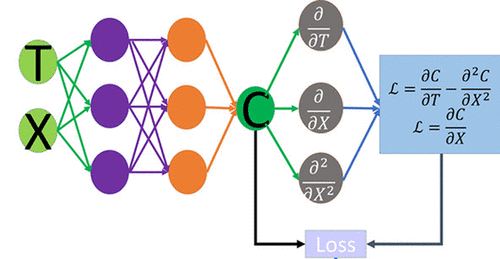
\includegraphics{PINN scheme.png}
%     \caption{Принципиальная схема работы PINN}
%     \label{fig:pinn_scheme}
% \end{figure}

\FloatBarrier
\subsection{Техническая реализация}
\subsubsection{Используемые технологии}

% В данном разделе обсудим технологии, необходимые для создания PINN

Для разработки будем использовать язык Python 3.10.6 -- высокоуровневый язык программирования общего назначения, один из наиболее популярных языков в области машинного обучения и Tensorflow -- библиотеку для создания и обучения нейронных сетей. Выбор данной библиотеки обусловлен простотой создания нейронных сетей с помощью Keras API, высокой производительностью, а так же встроенным автоматическим дифференцированием, которое и позволит нам обучить нейросеть дифференциальным уравнениям в частных производных.

\subsubsection{Програмная реализация PINN}

% Общая архитектура сети $\bar{u}(z)$, аппроксимирующей функцию $u(z)$ была описана в разделе \ref{sect:nn}, точное число слоёв и нейронов в каждом слое будем выбирать экспериментально, в качестве функции активации слоя будем использовать $\tanh$. Для создания нейронной сети воспользуемся классом \texttt{tensorflow.keras.Model}, слоёв классом \texttt{tensorflow.keras.layers.Dense}. PINN $f(x)$ будет иметь всего один слой. Параметрами этого слоя и есть параметры $\lambda_j$ из системы \eqref{eq:1syst}. На вход слой получает $N_f$ точек \eqref{eq:1syst} и $N_b$ точек для граничных условий. Внутри этого слоя мы считаем частные производные $u(x)$ с помощью \texttt{tensorflow.GradientTape}, и составлять из них и параметров $\lambda_j$ систему уравнений \eqref{eq:1syst}. На выход из данного слоя будем выдавать значения $u(z)$ и сами эти уравнения. В силу вида системы \eqref{eq:1syst} все выходы, соответствующие уравнениям системы \eqref{eq:1syst} должны быть равны 0. Как уже было сказано выше в качестве оптимизатора будем использовать Adam, а в качестве метрики MSE.

Общая архитектура сети $\bar{u}(z)$, аппроксимирующей функцию $u(z)$ была описана в разделе \ref{sect:nn}, в качестве функции активации слоя будем использовать $\tanh$. Для создания нейронной сети $\bar{u}$ воспользуемся классом tensorflow.keras.Model, слоёв классом tensorflow.keras.layers.Dense. Для удобства использования вынесем вычисление производных и функцию потерь в отдельную нейросеть-обёртку $f(\bar{u}, z)$. На вход сети $f$ подаём $N_f$ точек для системы \eqref{eq:1syst} и $N_b$ точек для граничных условий \eqref{eq:1bnd}. Для этих точек вычисляем значения $\bar{u}$, а так же её частные производные с помощью автоматического дифференцирования, реализуемого классом tensorflow.GradientTape. Затем составляем из них и параметров $\lambda_j$ систему уравнений \eqref{eq:1syst} и граничные условия \eqref{eq:1bnd}, они и будут являться выходами нейронной сети $f$. Функией потерь у $f$ будет \eqref{eq:pinn_loss}. Именно эту сеть мы будем обучать, при этом так как она включает в себя $\bar{u}$, то одновременно будет происходить и её обучение. Как уже было сказано в разделе \ref{sect:nn} в качестве оптимизатора будем использовать Adam, а в качестве метрики MSE.

% \setstretch{1.0}
% \begin{lstlisting}[language=Python]
% def build_net(layers, activation, dim, **kwargs):
%     ins = tf.keras.layers.Input(shape=(1+dim,))
%     z = ins
%     for layer in layers:
%         z = tf.keras.layers.Dense(layer, activation=activation,
%                                   kernel_initializer='he_normal')(z)

%     outs = {
%         "c": tf.keras.layers.Dense(1, kernel_initializer='he_normal')(z),
%         "Fi": tf.keras.layers.Dense(1, kernel_initializer='he_normal')(z),
%     }
%     return tf.keras.models.Model(inputs=ins, outputs=outs)
% \end{lstlisting}
% \setstretch{1.5}



\FloatBarrier
\section{Результаты и их обсуждение}

Все расчёты производились на процессоре 12th Gen Intel(R) Core(TM) i5-12400 2.50 GHz.

\subsection{Установившееся распределение тепла в кольце}

Рассмотрим для начала относительно простую задачу: определить распределение тепла, установившееся в кольце $1<r<2.\; 0<\phi<2\pi$, с граничными условиями:
\begin{equation}
    \begin{aligned}
        u(1,\phi)= & \cos\phi+\sin\phi+\sin(2\phi)+5\sin(3\phi)+1, \\
        u(2,\phi)= & \sin(2\phi)+\sin(3\phi)+\cos(4\phi).
    \end{aligned}
\end{equation}

Установившееся распределение тепла описывается уравнением Пуассона, учитывая что внутренних источников тепла нет получаем уравнение Лапласа:
\begin{equation}
    \Delta u = 0.
\end{equation}

Для полярных координат оно принимает вид

\begin{equation}
    \frac{\partial^2 u}{\partial r} + \frac{1}{r} \frac{\partial u}{\partial r} + \frac{1}{r^2}\frac{\partial^2 u}{\partial \phi^2} = 0.
\end{equation}

Данная задача имеет аналитическое решение:

\begin{equation}\label{eq:termal}
    \begin{split}
        u(r,\phi) & = 1-\frac{\ln r}{\ln 2}\\
        &+\brr{\frac{-r}{3}+\frac{4}{3r}}\sin(\phi)+\brr{\frac{-r}{3}+\frac{4}{3r}}\cos(\phi)\\
        &+\brr{\frac{r^2}{5}+\frac{4}{5r^2}}\sin(2\phi)\\
        &+\brr{\frac{3r^3}{63}+\frac{312}{64r^3}}\sin(3\phi)\\
        &+\brr{\frac{16r^4}{255}-\frac{16}{255r^4}}\cos(4\phi).
    \end{split}
\end{equation}

% Запустим обучение со следующими конфигурациями скрытых слоёв:
% \begin{itemize}
%     \item 20, 20, 20
%     \item 50, 50, 50
% \end{itemize}

% Для одной итерации обучения возьмём по одной точке для каждого граничного условия \eqref{eq:termal_cond} и одну внутреннюю точку для уравнения \eqref{eq:termal}, всего 3 точки на итерацию, точки выбираются случайным образом. Рассмотри случаи с 1000, 10000 и 100000 точек. Обучать будем в течении 1000 эпох или пока ошибка не будет улучшаться в течении 10 эпох хотя бы на 0.0001, размер батча 32. График обучения изображён на рисунке~\ref{fig:termal_loss}, время обучения указано в таблице \ref{table:termal_time}

% Для одной итерации обучения возьмём по одной точке для каждого граничного условия \eqref{eq:termal_cond} и одну внутреннюю точку для уравнения \eqref{eq:termal}, всего 3 точки на итерацию, точки выбираются случайным образом. Рассмотри случаи с количеством точек $N = 1000, 10000, 100000$. В каждом случае обучать будем в течении $10000000/N$, таким образом число итераций во всех случаях будет одинаково и можно будет оценить зависимость скорости обучения и итоговой точности от числа точек. Так же для сокращения времени обучения будем прерывать его, если в течении 1000 эпох не происходит улучшение функции потерь хотя бы на 0.0001. Размер батча 32 -- стандартный размер батча в \texttt{tensorflow}. График обучения изображён на рисунке~\ref{fig:termal_loss}, время обучения указано в таблице \ref{table:termal_time}

Для одной итерации обучения возьмём $N_f$ внутренних точек для уравнения \eqref{eq:termal} и $N_b$ точек для внутреннего и внешнего условий, обозначим их количество как $N_i$ и $N_o$ соответственно, всего $N_f+2N_b$ точек. В данном случае функция потерь будем выглядеть следующим образом:

\begin{equation}\label{eq:termal_cond}
    \begin{split}
        MSE =& \frac{1}{N_f}\sum_{i=1}^{N_f} \brr{\frac{\partial^2 u}{\partial r}(r_i, \phi_i) + \frac{1}{r} \frac{\partial u}{\partial r}(r_i, \phi_i) + \frac{1}{r^2}\frac{\partial^2 u}{\partial \phi^2}(r_i, \phi_i)}^2 + \\
        & \frac{1}{N_i}\sum_{i=1}^{N_i} \brr{u(1, \phi_i) - \cos\phi+\sin\phi+\sin(2\phi_i)+5\sin(3\phi_i) + 1}^2 + \\
        & \frac{1}{N_o}\sum_{i=1}^{N_o} \brr{u(2, \phi_i) - \sin (2\phi_i) +\sin(3\phi_i)+\cos(4\phi_i)}^2.
    \end{split}
\end{equation}

Возьмём за основу архитектуры сеть из \cite{bib:pinn:first}, но в место 8 слоёв оставим 4 слоя по 20 нейронов и проведём вычисления при различных значениях для $N_f$ и $N_b$. Эпох 10000. Валидацию буем проводить следующим образом: для уравнения~\eqref{eq:termal} разобьём область на радиальную сетку, с числом узлов $N_f$, для граничных условий~\eqref{eq:termal_cond} равномерно расположим на $[0, 2\pi]$ $N_b$ точек.

По графикам обучения, изображённым на рисунке~\ref{fig:termal_loss} видно, что при малом количестве внутренних точек $N_f$ значения функции потерь на валидационной выборке в несколько раз больше значений функции потерь на обучающей выборке, с увеличением $N_f$ же значения функции потерь на обучающей и валидационной выборках практически совпадаю.

\begin{figure}[htb!]
    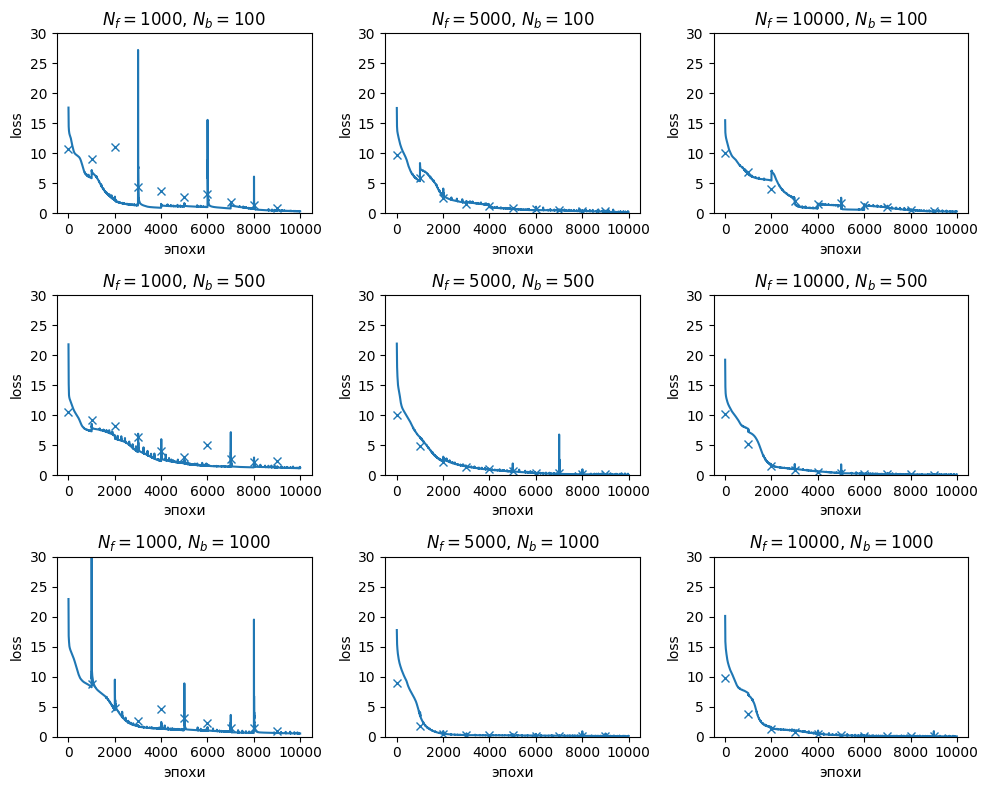
\includegraphics[width=\textwidth]{../plots/termal/loss l = (20x4) Nf=[1000, 5000, 10000] Nu=[100, 500, 1000].png}
    \caption{Графики функций потерь для различных сочетаний $N_f$ и $N_b$, крестиками изображаются результаты валидации в определённые моменты времени}
    \label{fig:termal_loss}
\end{figure}

% \begin{table}[htb]
%     \center
%     \begin{tabular}{|c|c|c|c|}
%         \hline
%         \diagbox{$N_f$}{$N_b$} & 1000 & 5000 & 10000\\
%         \hline
%         1000 & 10.06 & 85.62 & 401.14\\ 
%         \hline
%         50000 & 12.68 & 51.69 & 173.97\\
%         \hline
%         100000 & 12.68 & 51.69 & 173.97\\
%         \hline
%     \end{tabular}
%     \caption{Лучшее значение валидации для различных сочетаний $N_f$ и $N_b$}
%     \label{table:termal_loss}
% \end{table}

% \begin{table}[htb]
%     \center
%     \begin{tabular}{|c|c|c|c|}
%         \hline
%         \diagbox{Слои}{Итераций} & 1000 & 10000 & 100000\\
%         \hline
%         [20, 20, 20] & 10.06 & 85.62 & 401.14\\
%         \hline
%         [50, 50, 50] & 12.68 & 51.69 & 173.97\\
%         \hline
%     \end{tabular}
%     \caption{Время обучения в секундах}
%     \label{table:termal_time}
% \end{table}

Время обучения, указанное в таблице \ref{table:termal_time} практически не зависит от количества точек для граничных условий $N_b$, вероятно потому что с ними не производится вычисление производных, а так же потому что их в целом меньше. В целом время обучения получается достаточно большим, возможным решением данной проблемы может быть изменение числа слоёв и количества нейронов в слоях.

\begin{table}[H]
    \center
    \begin{tabular}{|c|c|c|c|}
        \hline
        \diagbox{$N_b$}{$N_f$} & 1000   & 5000    & 10000   \\
        \hline
        100                    & 311.65 & 1108.51 & 3494.39 \\
        \hline
        500                    & 314.31 & 1112.09 & 3487.54 \\
        \hline
        1000                   & 312.27 & 1109.55 & 3472.66 \\
        \hline
    \end{tabular}
    \caption{Время обучения в секундах для различных сочетаний $N_f$ и $N_b$}
    \label{table:termal_time}
\end{table}

Выполнение граничных условий при различных $N_b$ изображено на рисунках \ref{fig:termal_bnd1}, \ref{fig:termal_bnd2}, \ref{fig:termal_bnd3}. Для всех случаев характерно то, что внутренне условие при $r=1$ выполняется почти идеально, исключение составляет случай $N_f=1000, N_b = 500$, у которого изгибается конец. Внешнее условие однако выполняется относительно плохо. Связанно такое различие вероятнее всего с тем, что разброс величин у внутреннего условия больше -- от -4 до 8, в то время как у внешнего в два раза меньше от -3 до 2, для решения данной проблемы в дальнейшем можно попробовать внести весовой коэффициент для граничного условия равный $\frac{1}{\max_\phi{u(r_0, \phi)}}$.

% \begin{figure}
%     \begin{subfigure}[b]{0.32\textwidth}
%         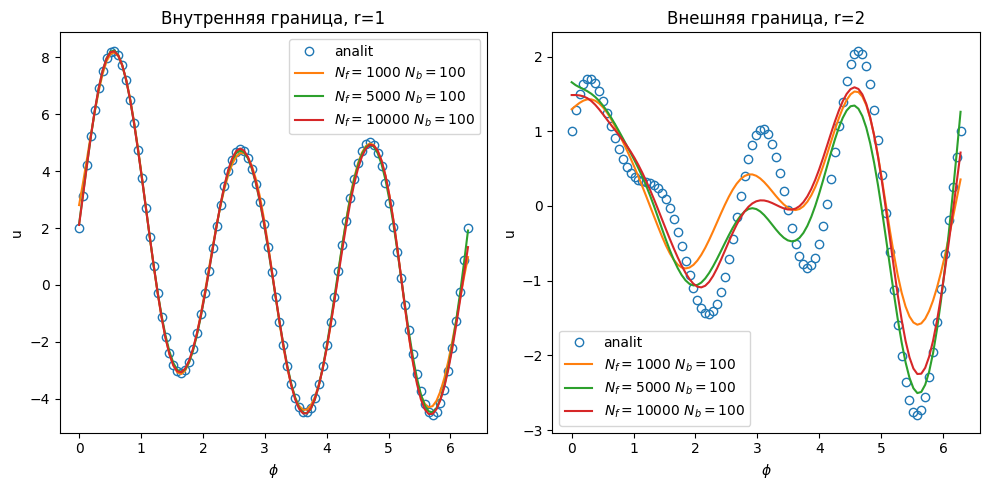
\includegraphics[width=\textwidth]{../plots/termal/bnd l = (20x4) Nf=[1000, 5000, 10000] Nu=100.png}
%     \end{subfigure}
%     \hfil
%     \begin{subfigure}[b]{0.32\textwidth}
%         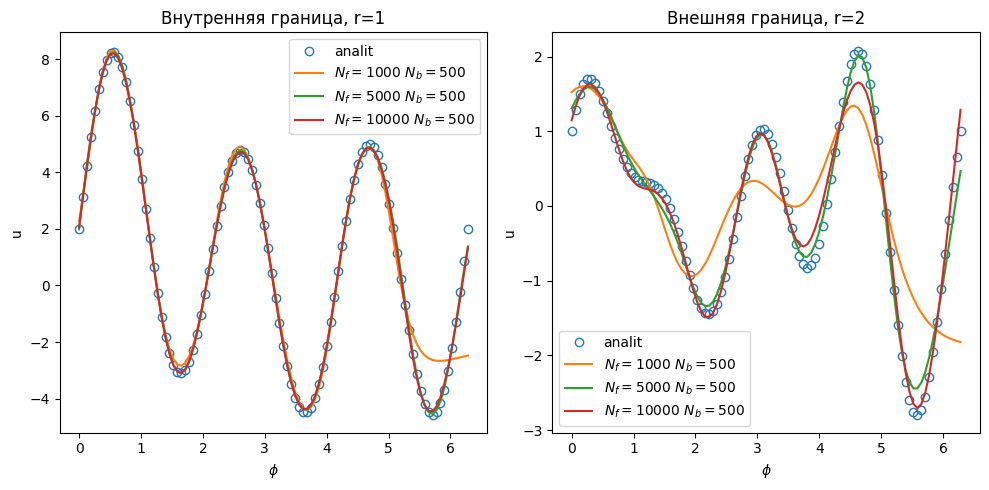
\includegraphics[width=\textwidth]{../plots/termal/bnd l = (20x4) Nf=[1000, 5000, 10000] Nu=500.png}
%     \end{subfigure}
%     \hfill
%     \begin{subfigure}[b]{0.32\textwidth}
%         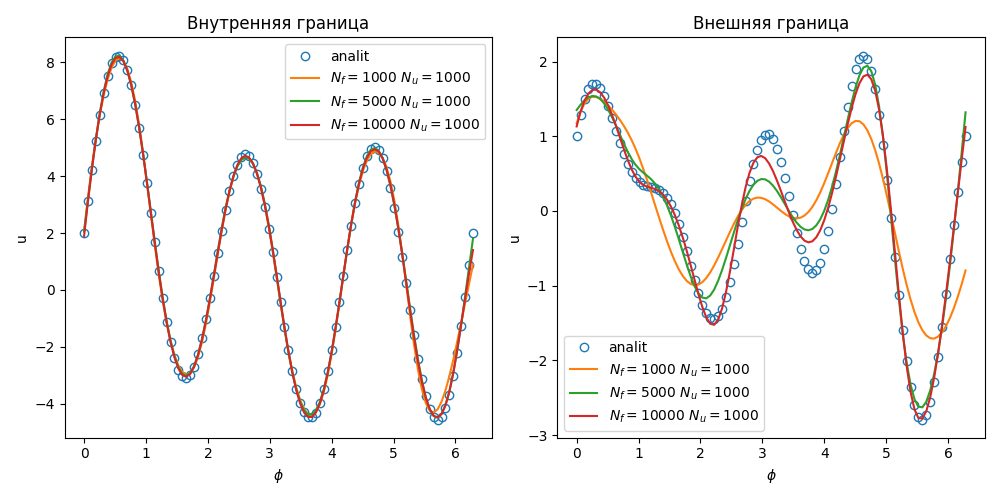
\includegraphics[width=\textwidth]{../plots/termal/bnd l = (20x4) Nf=[1000, 5000, 10000] Nu=1000.png}
%     \end{subfigure}
% \end{figure}

\begin{figure}[ht]
    \center
    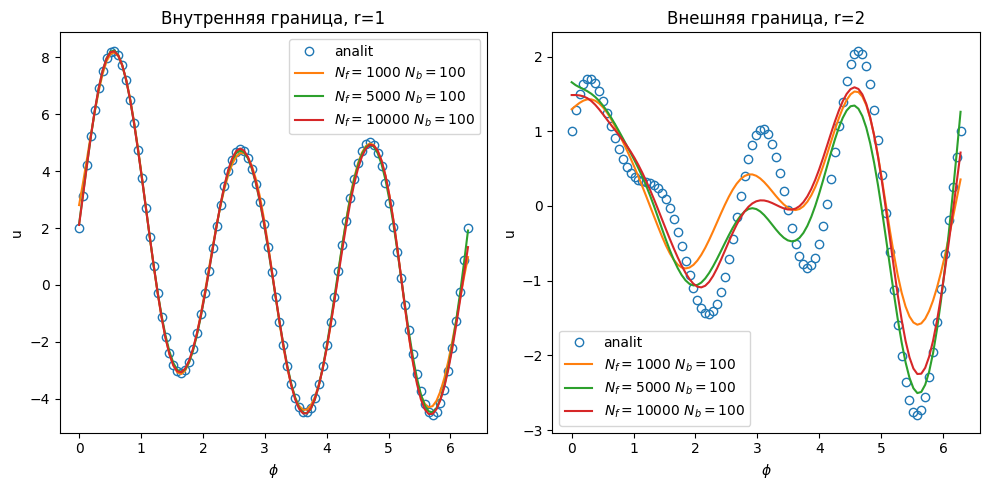
\includegraphics[width=0.7\textwidth]{../plots/termal/bnd l = (20x4) Nf=[1000, 5000, 10000] Nu=100.png}
    \caption{Граничные условия для случая $N_b=100$}
    \label{fig:termal_bnd1}
\end{figure}
\begin{figure}[ht]
    \center
    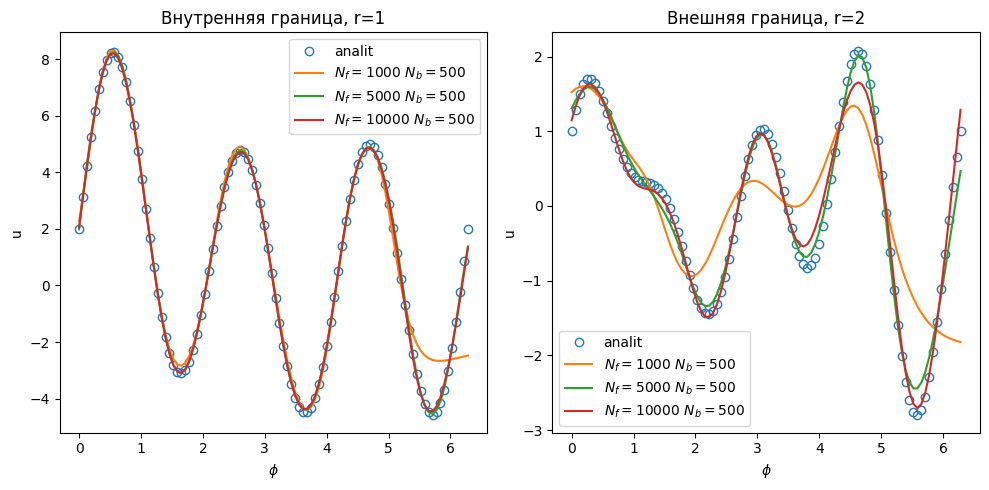
\includegraphics[width=0.7\textwidth]{../plots/termal/bnd l = (20x4) Nf=[1000, 5000, 10000] Nu=500.png}
    \caption{Граничные условия для случая $N_b=500$}
    \label{fig:termal_bnd2}
\end{figure}
\begin{figure}[ht]
    \center
    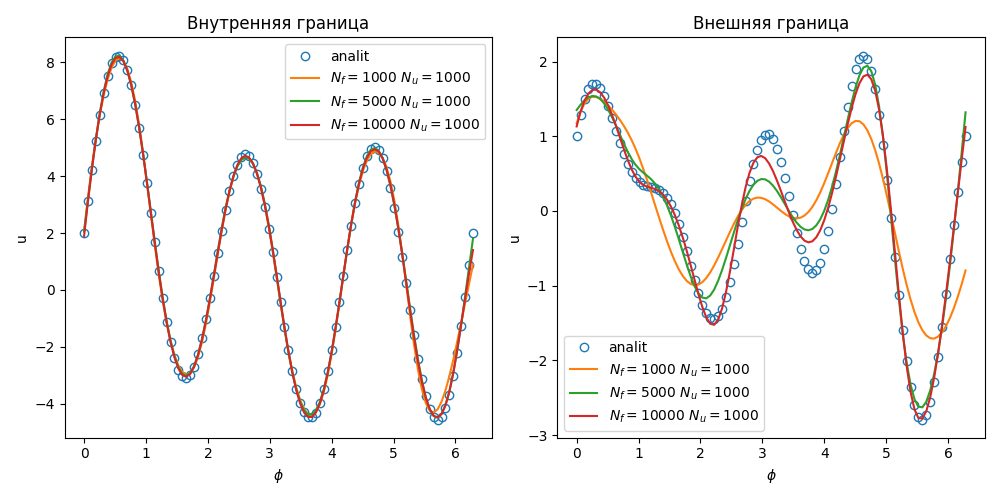
\includegraphics[width=0.7\textwidth]{../plots/termal/bnd l = (20x4) Nf=[1000, 5000, 10000] Nu=1000.png}
    \caption{Граничные условия для случая $N_b=1000$}
    \label{fig:termal_bnd3}
\end{figure}
\FloatBarrier

% Как видно из графика~\ref{fig:termal_loss} число нейронов в слое не оказывает существенного влияния на сходимость и точность сети, в то время как количество точек оказывает.

% Точки для обучения возьмём по $N$ точке для граничных условий и ещё $N$ точек для внутренних, всего $3N$ точек, где $N = 1000, 10000, 10000$. Обучать будем в течении 1000 эпох или пока ошибка не будет улучшаться в течении 10 эпох хотя бы на 0.001, размер батча.

% \subsection{Задача электрокинетики}

Для примера возьмём систему из \cite{bib:tutor}. Она описывается следующими уравнениями
$$\begin{aligned}
        \vec{j}                                                               & =
        -D \nabla c - \xi z e c \nabla \Phi + c \vec{u}                                    \\
        \partial_{t} c                                                        & =
        -\nabla \cdot\vec{j}                                                               \\
        \nabla^2 \Phi                                                         & =
        -4 \pi l_\mathrm{B} k_\mathrm{B}T z c                                              \\
        \rho \big( \partial_t \vec{u} + (\vec{u} \cdot \nabla ) \vec{u} \big) & =
        -\nabla p_H + \eta \nabla^{2} \vec{u} - (k_\mathrm{B}T \nabla c + zec \nabla \Phi) \\
        \nabla \cdot \vec{u}                                                  & =
        0
    \end{aligned}$$

Здесь первое уравнение в системе описывает поток плотности, второе электростатику, третье гидродинамику с помощью уравнения Навье-Стокса, четвёртое уравнение несжимаемости жидкости.

Рассмотрим систему щелевых пор, состоящую из двух одноимённо заряженных бесконечных пластин. Выпишем для такой системы граничные условия

$$
    \begin{aligned}
        c(t, X_l)       & = 0.01        \\
        c(t, X_r)       & = 0.01        \\
        c(0, X)         & = 0.002       \\
        \vec{v}(t, X_l) & = 0           \\
        \vec{v}(t, X_r) & = 0           \\
        \vec{v}(0, X)   & = 0           \\
        \Phi(t, X_l)    & = -0.05       \\
        \Phi(t, X_r)    & = -0.05       \\
        \Phi(0, X)      & = -0.009x^2+2
    \end{aligned}
$$
здесь $t$ -- время, $X_l$ -- пространственные координаты, соответствующие левой стенке, $X_r$ -- правой, $x$ в формул для $\Phi(0,x)$ соответствует оси, перпендикулярной пластинам.

\subsection{Упрощённый случай}

В начале рассмотрим упрощённую систему уравнений с одной пространственной координатой и без скорости

$$
    \begin{aligned}
        \frac{dc}{dT} & = -\nabla \cdot (- D\nabla c - \xi z e c \nabla \Phi) \\
        \nabla^2 \Phi & = -4 \pi l_\mathrm{B} k_\mathrm{B}T c
    \end{aligned}
$$

С граничными условиями

$$
    \begin{aligned}
        \frac{dc}{dX}(t, 0) & = 0 \\
        \frac{dc}{dX}(t, 1) & = 0 \\
        c(0, X)             & = 1 \\
        \Phi(0)             & = 1 \\
        \Phi(1)             & = 1 \\
    \end{aligned}
$$

Координаты в данном случае нормализованны

$$T = t/t_{\max},\;  X = (x+x_{\min})/x_{\max}$$

где $t_max$ -- время симуляции, $x_max$ -- размер системы по $x$-овой координате, $x_{\min}$ - координата левой стенки. Оператор $\nabla$ действует по пространственным координатам $\nabla = (\frac{d}{d X})$, все константы положим равными 1 и исключим $4\pi$ из второго уравнения.

Запустим обучение следующим образом: 100 запусков обучения (функция \texttt{fit}) по 10 эпох на 10000 наборах точек (внутренняя, граничная и начальная). Обучение заняло 2 минуты 48 секунд, значение функции потерь: $1.7378\cdot 10^{-5}$. Результаты симуляции представлены на рис.~\ref{fig:1d:simp:c} \ref{fig:1d:simp:Fi}:

\begin{figure}[ht]
    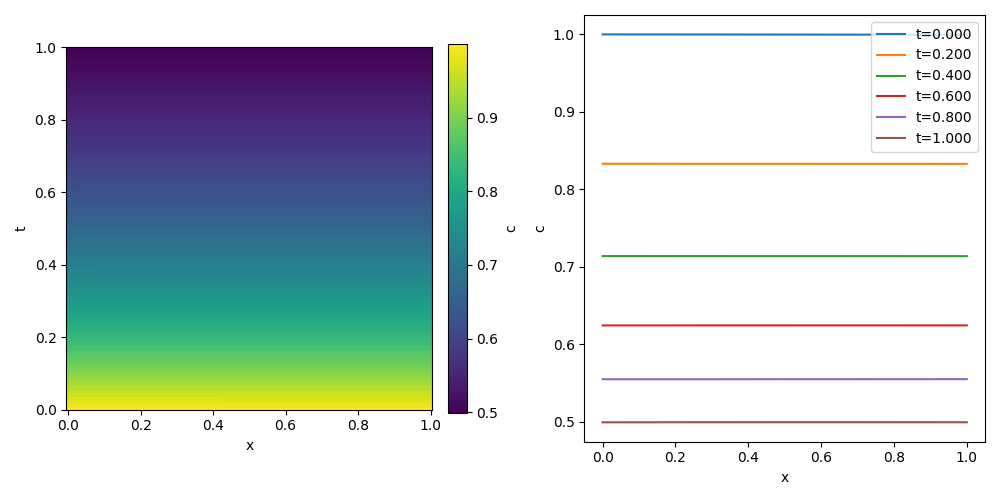
\includegraphics[width=\textwidth]{../plots/1-dim c simpified tanh 80,20.png}
    \caption{Упрощённый случай: концентрация}
    \label{fig:1d:simp:c}
\end{figure}

\begin{figure}[ht]
    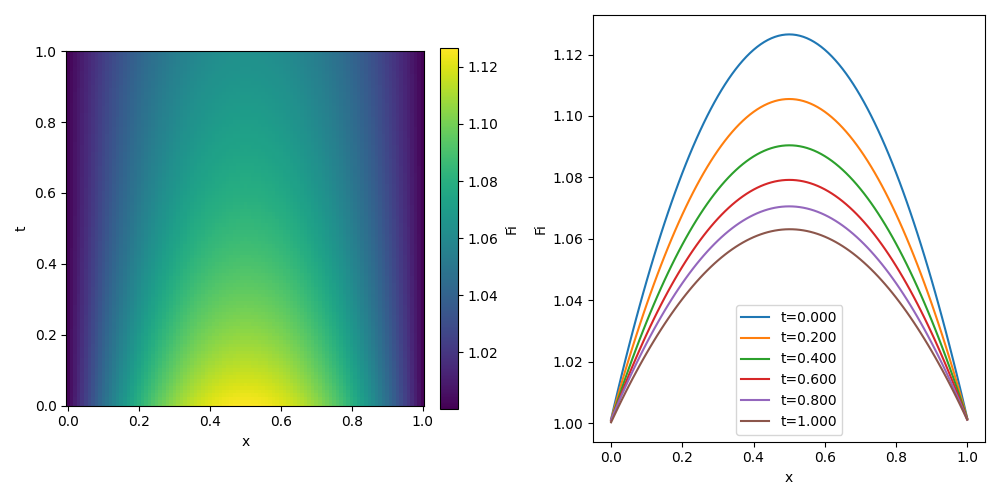
\includegraphics[width=\textwidth]{../plots/1-dim Phi simpified tanh 80,20.png}
    \caption{Упрощённый случай: потенциал}
    \label{fig:1d:simp:Fi}
\end{figure}

\subsection{Полный случай}

Рассмотрим двумерный случай. Скрытые слои будут иметь размеры 80 и 40, входной слой 4, один для концентрации, два для скорости и один для потенциала, функция активации $\tanh$ (гиперболический тангенс). Результат работы после 5000000 итераций показан на графике \ref{fig:2dres}

\begin{figure}[ht]
    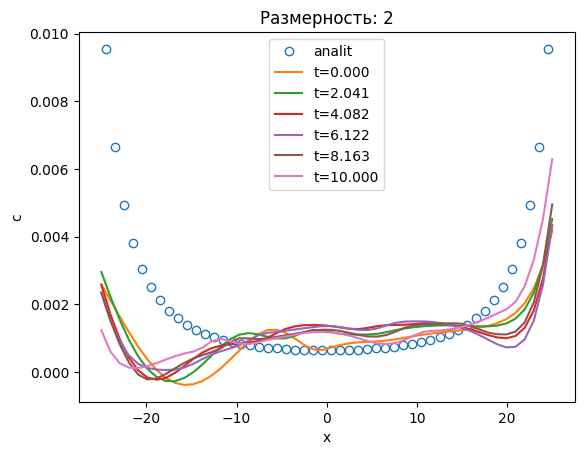
\includegraphics[scale=0.5]{../plots/2dim tanh 80 20.png}
    \caption{}
    \label{fig:2dres}
\end{figure}

Рассмотрим теперь трёхмерный случай. Скрытые слои так же будут иметь размеры 80 и 40, входной слой 5, один для концентрации, три для скорости и один для потенциала, функция активации $relu$. Результат работы после 30000000 итераций показан на графике \ref{fig:3dres}

\begin{figure}[ht]
    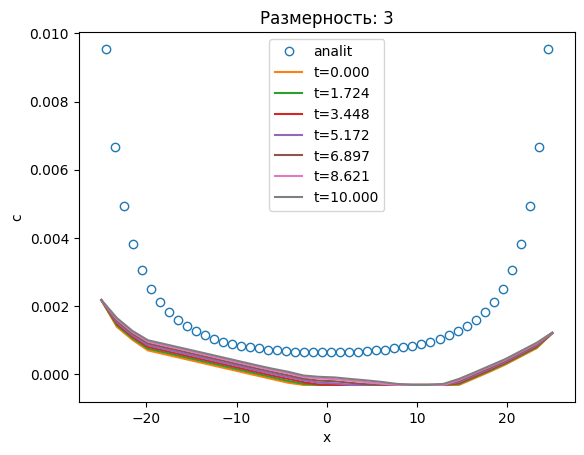
\includegraphics[scale=0.5]{../plots/3dim relu 80 20 30000000.png}
    \caption{}
    \label{fig:3dres}
\end{figure}

Наконец посмотрим на решение в целом. Точное решение изображено на графике~\ref{fig:termal_analit}, решение при различных $N_f$ и $N_b$ изображено на графике~\ref{fig:termal_pred}, ошибка между аналитическим решением и предсказаниями нейросети на графике~\ref{fig:termal_dif}. В целом графики достаточно хорошо совпадают в области. Расхождения наблюдаются в основном на стыке, где $\phi=0$. Что бы решить данную проблему можно попробовать добавить условие равенства $u(r, 0) = u(r, \phi)$, такому условию будет соответствовать следующая функция потерь:

\begin{equation}
    MSE_s = \frac{1}{N_s}\sum_{i=1}^{N_s} (u(r_i, 0) - u(r_i, 2\pi))^2,
\end{equation}
здесь $\brc{r_i}_{i=0}^{N_s}$ -- точки для данного условия, $N_s$ -- их количество.

\begin{figure}[ht]
    \center
    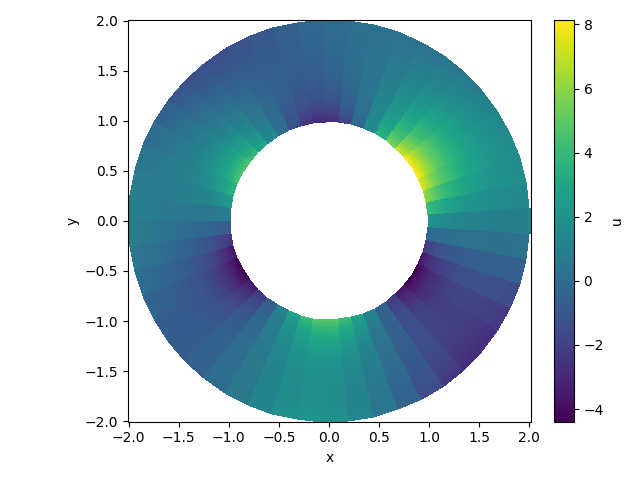
\includegraphics[width=0.5\textwidth]{../plots/termal/solut analit.png}
    \caption{Аналитическое решение}
    \label{fig:termal_analit}
\end{figure}

\begin{figure}[ht]
    \center
    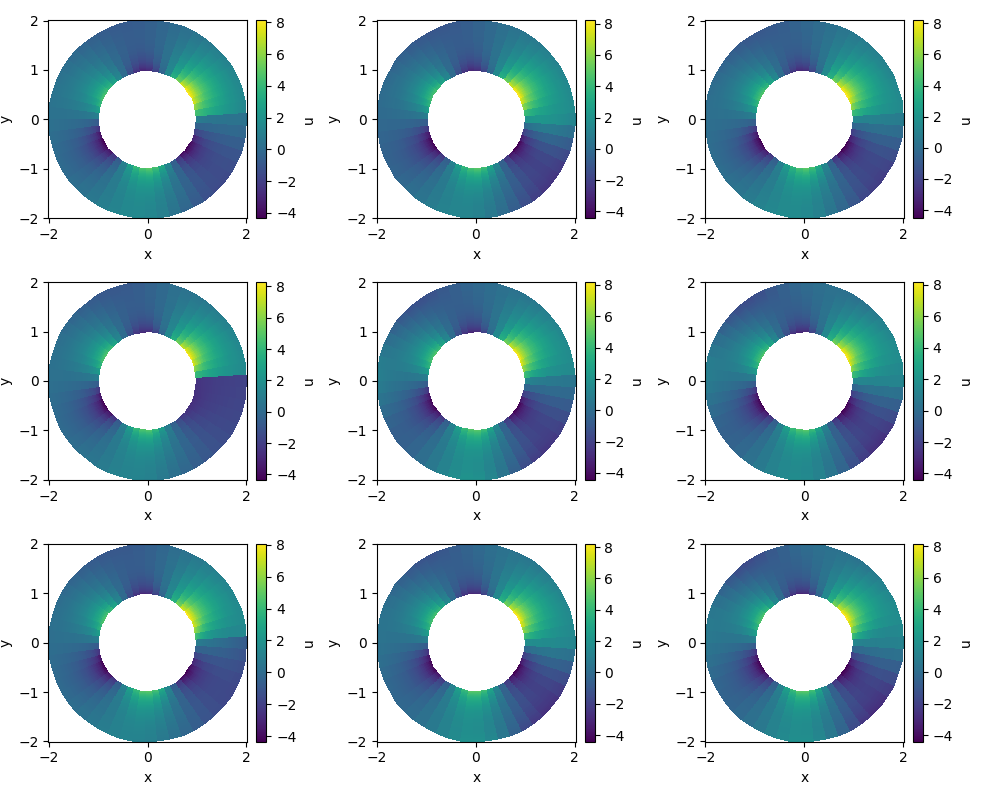
\includegraphics[width=\textwidth]{../plots/termal/solut l = (20x4) Nf=[1000, 5000, 10000] Nu=[100, 500, 1000].png}
    \caption{Решение при различных $N_f$ и $N_b$}
    \label{fig:termal_pred}
\end{figure}

\begin{figure}[ht]
    \center
    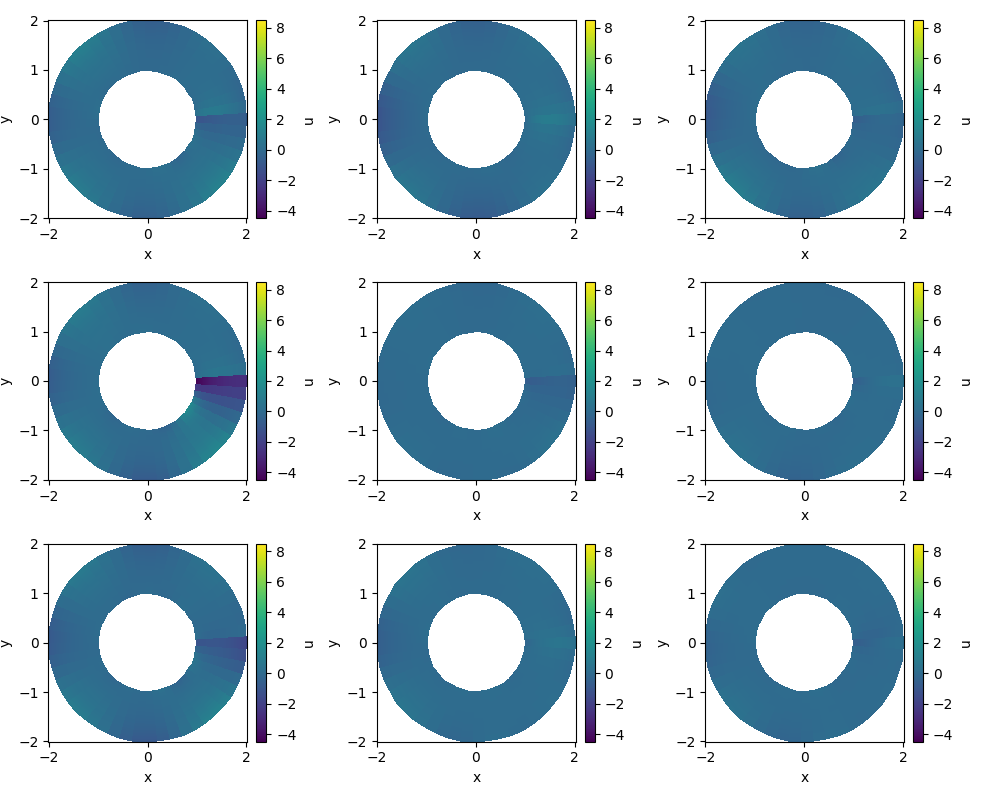
\includegraphics[width=\textwidth]{../plots/termal/solut dif l = (20x4) Nf=[1000, 5000, 10000] Nu=[100, 500, 1000].png}
    \caption{Разница между аналитическим решением и решением нейросети при различных $N_f$ и $N_b$}
    \label{fig:termal_dif}
\end{figure}

\FloatBarrier
\subsection{Задача электрокинетики}

В качестве второго примера возьмём систему из \cite{bib:tutor}. Она описывается следующими уравнениями
\begin{equation}\label{eq:ek_eq}
    \begin{aligned}
        \vec{j}                                             & =
        -D \nabla c - \xi z e c \nabla \Phi + c v,                                    \\
        %
        \partial_{t} c                                      & =
        -\nabla \cdot\vec{j},                                                         \\
        %
        \nabla^2 \Phi                                       & =
        -4 \pi l_\mathrm{B} k_\mathrm{B}T z c,                                        \\
        %
        \rho \big( \partial_t v + (v \cdot \nabla ) v \big) & =
        -\nabla p_H + \eta \nabla^{2} v - (k_\mathrm{B}T \nabla c + zec \nabla \Phi), \\
        %
        \nabla \cdot v                                      & =
        0,
    \end{aligned}
\end{equation}
здесь $c$ -- концентрация ионных частиц, $j$ -- поток плотности, $\vec{v}$ -- адвективная скорость жидкости, $e$ -- заряд электрона $z$ -- валентность частиц, $\Phi$ -- электростатический потенциал, $\xi$ -- подвижность частиц, $D$ -- коэффициент диффузии частиц, $l_B$ -- длина Бьеррума, $l_B = \frac{e^2}{4\pi\varepsilon k_B T}$ $k_B$ -- постоянная Больцмана, $T$ -- температура, $\rho$ -- плотность жидкости $p_H$ -- гидродинамическое давление. Первое уравнение в системе описывает поток плотности, второе электростатику, третье гидродинамику с помощью уравнения Навье-Стокса, четвёртое уравнение несжимаемости жидкости. В данном случае $z = (t, X)$ t -- время, X -- пространственные координаты.

Размерности для величин так же возьмём из \cite{bib:tutor}:

\begin{table}[H]
    \center
    \begin{tabular}{|l|l|}
        \hline
        Величина & Единица симуляции в единицах СИ \\
        \hline
        Длина    & 1нм                             \\
        \hline
        Энергия  & $4.14\cdot 10^{-21}$ Дж         \\
        \hline
        Масса    & $3.28 \cdot 10^{-26}$ кг        \\
        \hline
        Время    & $3.04 \cdot 10^{-12}$ с         \\
        \hline
        Заряд    & $1.60 \cdot 10^{-19}$ Кл        \\
        \hline
    \end{tabular}
    \caption{Единицы измерения симуляции в единицах измерения СИ}
\end{table}

Рассмотрим систему щелевых пор, состоящую из двух одноимённо заряженных бесконечных пластин. Выпишем для такой системы граничные условия

\begin{equation}\label{eq:ek_bnd}
    \begin{aligned}
        c(t, X_l)    & = 0.01         \\
        c(t, X_r)    & = 0.01         \\
        c(0, X)      & = 0.002        \\
        v(t, X_l)    & = 0            \\
        v(t, X_r)    & = 0            \\
        v(0, X)      & = 0            \\
        \Phi(t, X_l) & = -0.05        \\
        \Phi(t, X_r) & = -0.05        \\
        \Phi(0, X)   & = -0.009x^2+2,
    \end{aligned}
\end{equation}
здесь $t$ -- время, $X_l$ -- пространственные координаты, соответствующие левой стенке, $X_r$ -- правой, $x$ в формул для $\Phi(0,X)$ соответствует оси, перпендикулярной пластинам.

В данной системе мы имеем 3 неизвестные -- концентрацию $c$, скорость $v$ и потенциал $\Phi$, соответственно наша сеть $\bar{u}(t, X)$ будет иметь три выхода $\bar{c}(t, X)$, $\bar{v}(t, X)$ и $\bar{\Phi}(t, X)$. Составим функцию потерь. Из системы~\eqref{eq:ek_eq} получаем:

\begin{equation}\label{eq:ek_mse_eq}
    \begin{aligned}
        MSE_f & = \sum_{i=1}^{N_f}\brs{\partial_{t} \bar{c}_i + \nabla\cdot(-D \nabla \bar{c}_i - \xi z e \bar{c}_i \nabla \bar{\Phi}_i + \bar{c}_i \bar{v}_i)}^2                                                                                  \\
              & +\sum_{i=1}^{N_f}\brs{\nabla^2 \bar{\Phi}_i + 4 \pi l_\mathrm{B} k_\mathrm{B}T z \bar{c}_i}^2                                                                                                                                      \\
              & \begin{aligned}
                    +\sum_{i=1}^{N_f} & \left[\rho \big( \partial_t \bar{v}_i + (\bar{v}_i \cdot \nabla ) \bar{v}_i \big) + \nabla p_H - \eta \nabla^{2} \bar{v}_i\right. \\
                                      & \left. +(k_\mathrm{B}T \nabla \bar{c}_i + ze\bar{c}_i \nabla \bar{\Phi}_i)\right]^2
                \end{aligned} \\
              & +\sum_{i=1}^{N_f}\brs{\nabla \cdot \bar{v}_i}^2.
    \end{aligned}
\end{equation}

Из граничных условий~\eqref{eq:ek_bnd} получаем

\begin{equation}\label{eq:ek_mse_bnd}
    \begin{aligned}
        MSE_b & = \sum_{i=1}^{N_b}(\bar{c}_i - c_i)^2 + \sum_{i=1}^{N_b}(\bar{v}_i - v_i)^2 + \sum_{i=1}^{N_b}(\bar{\Phi}_i - c_i)^2.
    \end{aligned}
\end{equation}

В формулах \eqref{eq:ek_mse_eq} и \eqref{eq:ek_mse_bnd} $\bar{c}_i = \bar{c}(t_i, X_i)$, $\bar{v}_i = \bar{v}(t_i, X_i)$, $\bar{\Phi}_i = \bar{\Phi}(t_i, X_i)$.

Рассмотрим в начале двумерный случай. Скрытые слои как и в прошлом примере будут четыре по 20, входной слой 4, один для концентрации, два для скорости и один для потенциала, функция активации $\tanh$ (гиперболический тангенс). $N_f = 10000$ точек коллокации для \eqref{eq:ek_eq}, $N_b=1000$ для каждого из граничных условий \eqref{eq:ek_bnd}. Посмотрим на график обучения сети, изображённый на рисунке~\ref{fig:2dloss}, из него видно что 10000 эпох было явно много, рассмотрим участок с 100 по 1000 эпохи (рисунок~\ref{fig:2dloss_trim}). Из участка явно видно, что обучение прекратилось в районе 500-ой эпохи.

\begin{figure}[h]
    \begin{subfigure}{0.49\textwidth}
        \center
        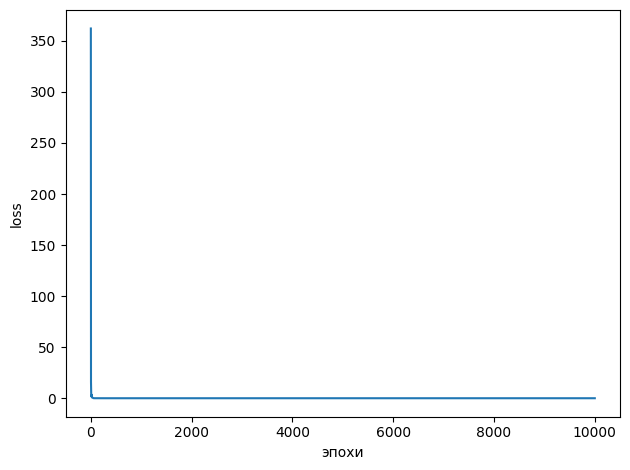
\includegraphics[width=\textwidth]{../plots/ek/2-dim loss 20x4.png}
        \caption{График обучения за все 10000 эпох}
        \label{fig:2dloss}
    \end{subfigure}
    \hfill
    \begin{subfigure}{0.49\textwidth}
        \center
        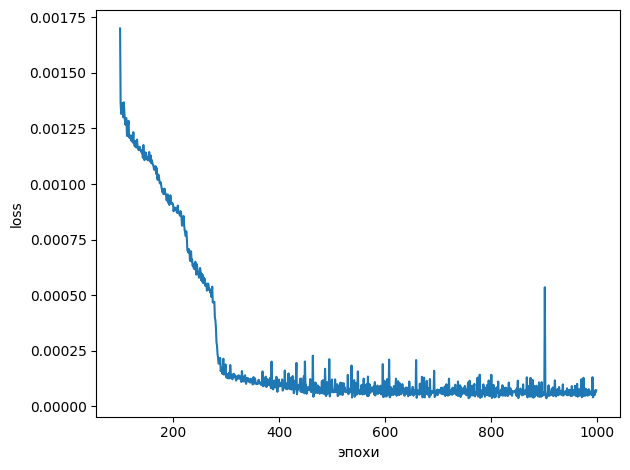
\includegraphics[width=\textwidth]{../plots/ek/2-dim loss trim20x4.png}
        \caption{График обучения c 100 по 1000 эпохи}
        \label{fig:2dloss_trim}
    \end{subfigure}
    \caption{Графики обучения для двухмерного случая электрокинетики для всех эпох и для участка от 100 до 1000}
\end{figure}

Сравним значения для концентрации $c$ полученные методом PINN и в ходе симуляции в \cite{bib:tutor} (рис.~\ref{fig:2dres}). Так как система приходит к стабильному состоянию, рассмотрим именно его. Судя по графику, нейросеть просто нашла нулевое решение, которое удовлетворяет системе \eqref{eq:ek_eq}, а на краях дотянула до граничных условий \eqref{eq:ek_bnd}.

\begin{figure}[H]
    \center
    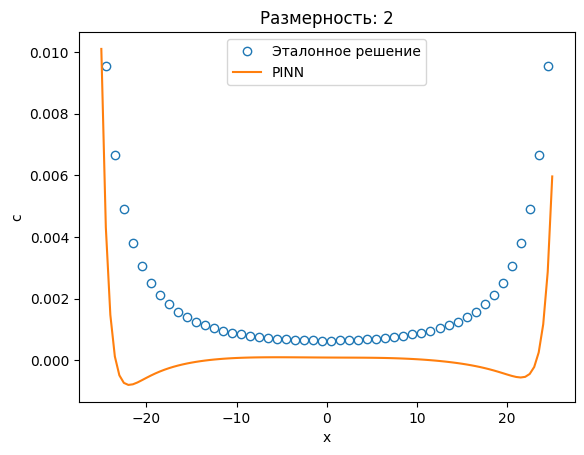
\includegraphics[scale=0.5]{../plots/ek/2-dim tanh 20x4.png}
    \caption{Концентрация c для двумерного случая}
    \label{fig:2dres}
\end{figure}

Рассмотрим теперь трёхмерный случай. Скрытые слои так же будут 4 по 20, входной слой 5, один для концентрации, три для скорости и один для потенциала, функция активации $\tanh$. $N_f = 10000$ точек коллокации для \eqref{eq:ek_eq}, $N_b=1000$ для каждого из граничных условий \eqref{eq:ek_bnd}. Посмотрим на график обучения сети, изображённый на рисунке~\ref{fig:3dloss}, из него видно что, как и в прошлом примере 10000 эпох было явно много, рассмотрим участок с 100 по 1000 эпохи (рисунок~\ref{fig:3dloss_trim}). Из участка видно, что обучение так же прекратилось в районе 500-ой эпохи.

\begin{figure}[h]
    \begin{subfigure}{0.49\textwidth}
        \center
        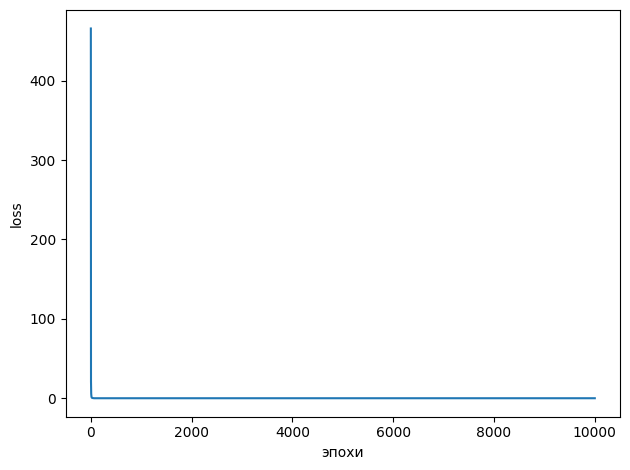
\includegraphics[width=\textwidth]{../plots/ek/3-dim loss 20x4.png}
        \caption{График обучения за все 10000 эпох}
        \label{fig:3dloss}
    \end{subfigure}
    \hfill
    \begin{subfigure}{0.49\textwidth}
        \center
        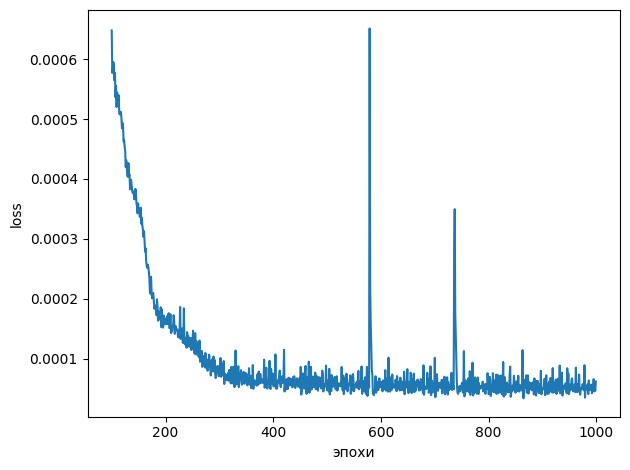
\includegraphics[width=\textwidth]{../plots/ek/3-dim loss trim20x4.png}
        \caption{График обучения c 100 по 1000 эпохи}
        \label{fig:3dloss_trim}
    \end{subfigure}
    \caption{Графики обучения для трёхмерного случая электрокинетики для всех эпох и для участка от 100 до 1000}
\end{figure}
Сравним значения для концентрации $c$ полученные методом PINN и в ходе симуляции в \cite{bib:tutor} (рис.~\ref{fig:3dres}). Так как система приходит к стабильному состоянию, рассмотрим именно его. В трёхмерном случае так же ожидаемо ен получилось получить хорошее приближение, вероятно как и в двумерном случае сеть нашла нулевое решение и застряла в нём.

\begin{figure}[H]
    \center
    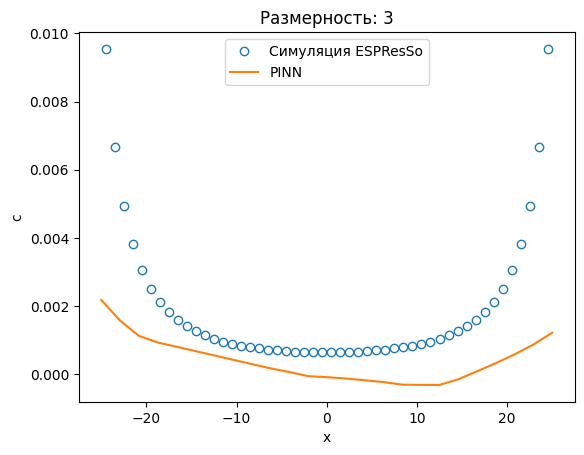
\includegraphics[scale=0.5]{../plots/ek/3-dim tanh 20x4.png}
    \caption{Концентрация c для трёхмерного случая}
    \label{fig:3dres}
\end{figure}

Как можно видеть из двух примеров достаточно сложные системы на данный момент плохо поддаются решению с помощью PINN.

\newpage
\FloatBarrier
\newpage
\FloatBarrier
\begin{center}
    \section*{ЗАКЛЮЧЕНИЕ}
    \addcontentsline{toc}{section}{ЗАКЛЮЧЕНИЕ}
\end{center}

В ходе работы мы написали, обучили и протестировали две PINN, для двух задач математической физики. Для первой задачи -- распределение тепла в кольце нам удалось получить в целом достаточно хорошее решение, близкое к истинному. Во второй задаче с электрокинетикой у нас уже не получилось получить результаты, близкие к истинным.

Возможные улучшения:

\begin{enumerate}[label={\arabic*)}]
    \item Подобрать весовые коэффициенты для функций потерь
    \item Поэкспериментировать с числом слоёв и нейронов в каждом слое
    \item Добавить дополнительное условие, требующее равенства на границе при $\phi=0, 2\pi$
\end{enumerate}

\newpage
\begin{center}
    \section*{СПИСОК ИСПОЛЬЗОВАННЫХ ИСТОЧНИКОВ И ЛИТЕРАТУРЫ}
    \label{sec:intro}
    \addcontentsline{toc}{section}{\nameref{sec:intro}}
\end{center}
\renewcommand{\refname}{}
\vglue-40pt
\bibliographystyle{unsrt}
\bibliography{otchet}

\end{document}